\documentclass[11pt]{article}
\usepackage{times,epsfig,subcaption,wrapfig,algorithmic,color,boxedminipage,graphicx,url}
\usepackage{authblk}
\setlength{\affilsep}{0em}
\usepackage{debulletin}
\usepackage{etoolbox, totcount}
\usepackage{import}
\usepackage{xcolor}
\usepackage{authblk}
\usepackage{microtype}
\usepackage{multirow,url,amsmath,amsfonts,amsfonts,xspace}
\usepackage{hyperref}

\usepackage[color,matrix,arrow,all]{xy}
\usepackage{tikz}
\usetikzlibrary{shapes,decorations}
\usetikzlibrary{calc}



\usepackage[english]{babel}
\usepackage[utf8]{inputenc}
\usepackage{enumitem,kantlipsum}
\usepackage{graphicx, color}
\usepackage{wrapfig}
\usepackage{amsfonts}


%removed subfigure which is deprecated --> switch to subcaption

% this is the template for an issue of the Data Engineering Bulletin

% all packages used by any paper must be listed here
\usepackage{listings}
\usepackage{caption}

\usepackage{listings}
\usepackage{booktabs}
\usepackage{listings}
\usepackage{xargs}
%\PassOptionsToPackage{hyphens}{url}
%\usepackage{hyperref}
\usepackage{multirow}
\usepackage{tabularx}
\usepackage{makecell}
\usepackage{arydshln}
\usepackage{xspace}
\usepackage{tcolorbox}
\usepackage{xpatch}

% Added for better import behavior
\usepackage{import}

% Added for covista paper
\usepackage{etoolbox, totcount}


\newcommand{\Hypercallback}{Hyperupcall\xspace{}}
\newcommand{\hypercallback}{hyperupcall\xspace{}}
\newcommand{\hide}[1]{}

\def\UrlBreaks{\do-\do\.\do\@\do\\\do\!\do\_\do\|\do\;\do\>\do\]\do\)\do\,\do\?\do\'\do+\do\=\do\#}
\def\UrlBigBreaks{\do\:\do\/}



\begin{document}


% please enter real date, vol no, issue no
\bulletindate{June 2020}
\bulletinvolume{43}
\bulletinnumber{2}
\bulletinyear{2020}

% these are files that I have- but your part of the issue can be done without
% them
\IEEElogo{cs.pdf}
\insidefrontcover{incvA19.pdf}
%\insidebackcover[ICDE Conference]{./calls/icde-new-a.ps}

\begin{bulletin}

% the above samples assume the issue is generated from a directory structure of the following sort
% major directory name is month and year of issue
% there are sub-directorys for
% letters: directory name is "letters"
% technical articles: a directory per paper, named for an "author"
% news articles: directory name is "news"
% calls: directory name is "calls

%
%  Editor letters section.  Use the lettersection environment.
%  Each letter is contained in a letter environment, where the two required
%  options to \begin{letter} are the author and the address of the author.
%

\begin{lettersection}

% there will be other letters- and a blank page will appear in your document
% but the special issue part will be fine

\begin{letter}{Letter from the Editor-in-Chief}
{Haixun Wang}{WeWork Corporation}
\documentclass[11pt]{article} 

\usepackage{deauthor,times,graphicx}
%\usepackage{url}
\usepackage{hyperref}

\begin{document}
Around the time we published our last issue in March, the nation went
into a lockdown. Life in the last 3 months has been unprecedented in
many ways. As governments around the world scrambled to fight
coronavirus, people in the scientific community, especially those on
the frontline -- doctors, healthcare professionals, medical staff and
researchers -- made heroic efforts and sacrifices to curb the pandemic
and save lives. The data management and data science communities also
sprang to action immediately. Globally, it is the first time that data
driven approaches are being used at such a large scale toward solving
a common problem. Under this backdrop, in this special issue of the
Data Engineering Bulletin edited by Joseph Gonzalez, we feature 8
papers on the topic of {\it digital contact tracing}, a technique that
may prove crucial in the fight against Covid-19.

This issue also features two opinion pieces. Divyakant Agrawal and Amr
El Abbadi's wake-up call on managing data in an untrusted environment
takes us to the fascinating world of cryptocurrencies and
blockchains. It shows what the database community, which was
responsible for creating and perfecting transaction management and
distributed systems, can learn from the blockchain approach when it
comes to handling untrusted behaviours from the underlying
infrastructure. The second opinion piece, written by Jeffrey
D. Ullman, addresses a question on the mind of every data management
person: What is our role in the machine learning and AI revolution?
Have we missed the boat again and become irrelevant? Ullman's
perspective, illustrated by his remake of the well known Conway Venn
Diagram that illustrates the relationship between computer science,
mathematics \& statistics, and domain knowledge is incisive,
thought-provoking, and entertaining at the same time.
\end{document}


\end{letter}
%
\newpage
%
%% your introductory letter goes here
%
\begin{letter}{Letter from the Special Issue Editor}
{Joseph Gonzalez}{University of California at Berkeley}
\documentclass[11pt]{article} 

\usepackage{deauthor,times,graphicx}
%\usepackage{url}
\usepackage{hyperref}



\begin{document}

Machine learning is rapidly maturing into an engineering discipline at the center of a growing range of applications.
This widespread adoption of machine learning techniques poses a new set challenges around the management of the data, code, models, and their relationship throughout the machine learning life-cycle.
In this issue of the Data Engineering Bulletin we have solicited work from both academic and industrial leaders in the data engineering community that are exploring how data engineering techniques can be used to address the challenges of the machine learning life-cycle.




\begin{figure}[h]
\centering
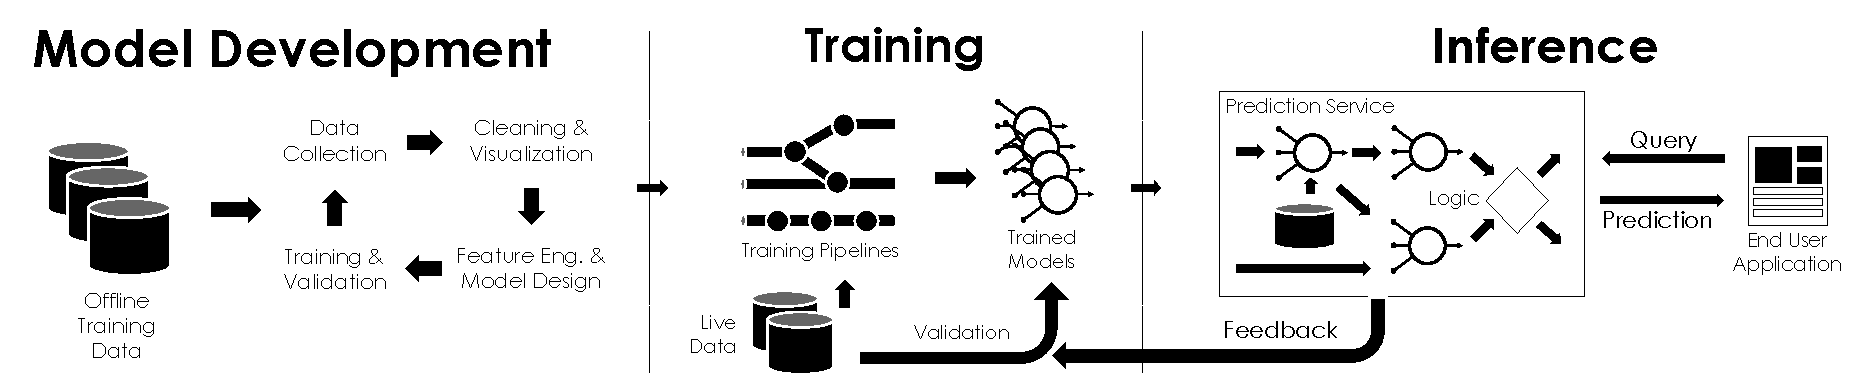
\includegraphics[width=\textwidth]{letters/pipeline.pdf}
\caption{\small \textbf{Machine Learning Life-cycle.} A simplified depiction of the key stages of a machine learning application.}
\label{fig:mllc}
\end{figure}


The machine learning life-cycle (Fig.~\ref{fig:mllc}) spans not only the model development, but also production training and inference.
Each stage demands different skills (e.g., neural network design, data management, and cluster management) and imposes different requirements on the underlying systems.
Yet there is an overwhelming need for unifying design principles and technologies to address pervasive problems including: feature management, data provenance, pipeline reproducibility, low-latency serving, and prediction monitoring just to name a few.


There has been substantial recent progress in systems to aid in managing the machine learning life-cycle.  
Large industrial projects like 
FB Learner Flow 
% \href{https://code.fb.com/core-data/introducing-fblearner-flow-facebook-s-ai-backbone/}{FB Learner Flow}
from Facebook, 
Michelangelo 
% \href{https://eng.uber.com/michelangelo/}{Michelangelo} 
from Uber, and 
TFX 
% \href{https://www.tensorflow.org/tfx/}{TFX} 
from Google have received a considerable of recent attention.  
In this issue we have solicited publications from several more recent industrial and academic projects.

The first paper, by a team at Amazon Research, provides an overview of several real-world use cases and then outlines the key conceptual, data management, and engineering challenges faced in production machine learning systems.
Rather than advocating a single system, this work describes some design principles that can inform potential solutions.


The second and third papers explores the challenges of model management and provenance across the machine learning life-cycle.
They motivate the need for systems to track models and their meta-data to improve reproducibility, collaboration, and governance. 
% expands upon the machine learning life-cycle 
% to include: data preparation, feature engineering, model training, deployment, and maintenance
% and explores the challenges of model 
The second paper introduces, ModelDB, an open-source system for model management and describe some of the functionality and design decisions. 
The third paper describes a related system, ProvDB, that uses a graph data model to capture and query fine-grained versioned lineage of data, scripts, and artifacts throughout the data analysis process.


The fourth paper, by a team at Databricks Inc., describes, MLFlow, a new open-source system to address the challenges of experimentation, reproducibility, and deployment. 
This work leverages containerization to capture the model development environment and a simple tracking API to enable experiment tracking.
The extensible model containerization enables model developers to more easily collaborate around modeling environments and then deploy model containers.


The last paper, by a team at Microsoft, focuses on inference and explores the challenges and opportunities of serving white-box prediction pipelines.  
In contrast to the containerization of pipelines in MLFlow, the Microsoft team leverage knowledge about the internal of the prediction pipeline to more efficient serve predictions. 



\end{document}




\end{letter}

\end{lettersection}

% put the name of your special issue below

\begin{opinionsection}
\begin{opinion}{Resurrecting Middle-Tier Distributed Transactions}
{Philip A. Bernstein}{Microsoft Research, Redmond, WA 98052}
\documentclass[11pt]{article} 
\usepackage{deauthor,times,graphicx,hyperref} 

\begin{document}
\title{Resurrecting Middle-Tier Distributed Transactions}
\author{Philip A. Bernstein\\Microsoft Research\\philbe@microsoft.com}


%\maketitle

\section{Introduction}
Over the years, platforms and application requirements change. As they do, technologies come, go, and return again as the preferred solution to certain system problems. In each of its incarnations, the technology's details change but the principles remain the same. One such technology is distributed transactions on middle-tier servers. Here, we argue that after a 15-year decline, they need to return to the mainstream. 

In the 1980's, Transaction Processing (TP) monitors were a popular category of middleware product that enabled customers to build scalable distributed systems to run transactions. Example products were CICS (IBM), Tuxedo (AT\&T for Unix), ACMS (DEC for VAX/VMS), and Pathway (Tandem for Guardian) \cite{4}. Their main features were multithreaded processes (not supported natively by most operating systems), inter-process communication (usually a crude form of remote procedure call), and a forms manager (for end users to submit transaction requests). The TP monitor ran on middle-tier servers that received transaction requests from front-end processors that communicated with end-user devices, such as terminals and PC's, and with back end database servers. The top-level application code executed on the middle-tier and invoked stored procedures on the database server.  
 
In those days, database management systems (DBMS's) supported ACID transactions, but hardly any of them supported distributed transactions. The TP monitor vendors saw this as a business opportunity and worked on adding a transaction manager feature that implemented the two-phase commit protocol (2PC). Such a feature required DBMS's to expose Start, Prepare, Commit, and Abort as operations that could be invoked by the TP monitor. Unfortunately, most of them didn't support Prepare, and even if they did, they didn't expose it to applications. They were willing to do so, but they didn't want to implement a different protocol for each TP monitor product. Thus, the XA standard was born, which defined TP monitor and DBMS interfaces (including Prepare) and protocols that allowed a TP monitor to run a distributed transaction across DBMS servers \cite{18}. 
 
This middle-tier architecture for distributed transactions was popular for about 20 years, into the late 1990s. Then TP monitors were replaced by Application Servers, which integrated a TP monitor with web servers, so it could receive transaction requests over HTTP, rather than receiving them from devices connected by a local area or terminal network. Examples include Microsoft Transaction Server, later renamed COM+, and Java Enterprise Edition (JEE), implemented by IBM's WebSphere Application Server, Oracle's WebLogic Application Server, and Red Hat's JBoss Application Server \cite{12}. The back end architecture was the same as before. Each transaction started executing on a middle-tier server and invoked stored procedures to read and write the database. 
 
Although this execution model is still widely used, starting in the early 2000's it fell out of favor for new application development, especially for applications targeted for cloud computing. More database vendors offered built-in support for distributed transactions, so there was less need to control the distributed transaction from the middle tier. A larger part of database applications executed on data that was cached in the middle tier. And the NoSQL movement argued that distributed transactions were too slow, that they limited scalability, and that customers rarely needed them anyway \cite{11}. Eventual consistency became all the rage \cite{19}. 
 
The critics of distributed transactions had some good points. But in the end, developers found that mainstream programmers really did need ACID transactions to make their applications reliable in the face of concurrent access to shared data and despite server failures. Thus, some NoSQL (key-value) stores added transaction support (e.g., CosmosDB \cite{2}, DynamoDB \cite{8}). Google, which had initially avoided support for multi-row distributed transactions in Bigtable \cite{5}, later introduced them in Spanner \cite{6}. There are now many cloud storage services and database products that support distributed transactions. 
 
Like product developers, database researchers have also focused on distributed transactions for back-end database systems. Almost universally, they assume that transactions execute as stored procedures and that middle-tier applications invoke those stored procedures but do not execute the transaction logic themselves. 
 
\section{Stateful Middle-Tier Applications}
This focus on stored procedures is well justified by the needs of traditional TP applications. However, stored procedures are not a good way of encapsulating application logic for a growing fraction of stateful applications that run on the middle tier. These include multi-player games, datacenter telemetry, Internet of Things, and social and mobile applications. Objects are a natural model for the entities in these applications, such as games, players, datacenter hardware, sensors, cameras, customers, and smart phones. Such applications have a large number of long-lived stateful objects that are spread over many servers and communicate via message passing. Like most new applications, these applications are usually developed to run on cloud computing platforms.  
 
These applications typically execute on middle-tier servers, rather than as stored procedures in database servers. They do this for many reasons. They need large main memory for the state of long-lived objects. They often have heavy computation needs, such as rendering images or computing over large graphs. They use a lot of computation for message passing between objects so they can scale out. And they need computation to be elastic, independent of storage requirements. These needs are satisfied by compute servers that are cheaper than database servers because they have less storage. Hence, these apps run on compute servers in the middle tier.  

\subsection{Requirements for Mid-Tier Cloud Transactions}
Some middle-tier applications need transactions because they have functions that read and write the state of two or more stateful objects. For example, a game may allow users to buy and sell virtual game objects, such as weapons, shields, and vehicles. A telemetry application may need to process an event exactly once by removing it from a queue and updating telemetry objects based on that event. A social application may need to add a user to a group and modify the user's state to indicate membership in that group. Each of these cases needs an ACID transaction over two or more objects, which may be distributed on different servers. Since these applications are usually developed to run on cloud computing platforms, distributed transaction support must be built into the cloud platform, a capability that is rarely supported today for cloud computing. 
 
Distributed transactions for middle-tier applications on a cloud computing platform have four requirements that differ from those supported by the late-1990's products that run transactions on the middle-tier. First, like all previous transaction mechanisms, they need to offer excellent performance. But unlike previous mechanisms, it's essential that they be able to scale out to a large number of servers, leading to the first requirement: The system must have high throughput and low transaction latency, at least when transactions have low contention, and in addition must scale out to many servers.  

To scale computation independently of storage, these applications typically save their state in cloud storage. The developers' choice of cloud storage service depends on their application's requirements (e.g., records, documents, blobs, SQL), their platform provider's offerings (e.g., AWS, Azure, Google), their employer's storage standards, and their developers' expertise. Thus, we have this second requirement: The transaction mechanism must support applications that use any cloud storage service.  

The transaction mechanism needs persistent storage to track transaction state: started, prepared, committed, or aborted. Like the apps themselves, it needs to use cloud storage for this purpose, which is the third requirement: The transaction mechanism must be able to use any of the cloud storage services used by applications. 

The traditional data structure for storing transaction state is a log. The transaction manager relies on the order of records in the log to understand the order in which transactions executed. Although cloud vendors implement logs to support their database services, they do not expose database-style logging as a service for customers, leading to a fourth requirement: The transaction mechanism cannot rely on a shared log, unless it implements the log itself, in which case the log must run on a wide variety of storage services. 
 
Due to the latency of cloud storage, requirements (2)-(4) create challenges in satisfying requirement (1). 

The above requirements are a first cut, based on today's applications and platforms. It is also worth targeting variations. For example, requirement (1) could include cost/performance, which might require a tradeoff against scalability. And (4) might go away entirely if cloud platforms offer high-performance logging as a service. 

\section{An Implementation in the Orleans Framework}
The rest of this paper sketches a distributed transaction mechanism that satisfies the above requirements \cite{9}. Our group built it for Microsoft's actor-oriented programming framework, called Orleans, which is open source and runs on both Windows and Linux \cite{16}. The distributed transaction project is part of a longer-term effort to enrich Orleans with other database features to evolve it into an actor-oriented database system that supports geo-distribution, stream processing, indexing, and other database features \cite{3}. 
\subsection{Two-Phase Commit and Locking}
For ACID semantics, Orleans transactions use two-phase commit (2PC) and two-phase locking (2PL). Our first challenge was to obtain high throughput and scalability despite the requirement to use cloud storage. In our runs, a write to cloud storage within a datacenter takes ~20 ms and has high variance. With 2PC, a transaction does two synchronous writes to storage. Therefore, if 2PL is used, a transaction holds locks for ~40ms, which limits throughput to 25 transactions/second (TPS). Low-latency SSD-based cloud storage is faster, but still incurs over 10 ms latency, plus higher cost. 
To avoid this problem, we extended early lock release to 2PC \cite{1,7,10,13,14,15}. After a transaction T1 terminates, it releases locks before writing to storage in phase one of 2PC. This allows a later transaction T2 to read/update T1's updated objects. Thus, while T1 is writing to storage, a sequence of later transactions can update an object, terminate, and then unlock the object. To avoid inconsistency, the system delays committing transactions that directly or indirectly read or overwrite T1's writeset until after T1 commits. And if T1 aborts, then those later dependent transactions abort too. Using this mechanism, we have seen transaction throughput up to 20x that of strict 2PL/2PC. 
\subsection{Logging}
Our initial implementation used a centralized transaction manager (TM) per server cluster \cite{9}. It ran on an independent server and was multithreaded. Since message-passing is a potential bottleneck, it batched its messages to transaction servers. It worked well with throughput up to 100K TPS. However, it had three disadvantages: it was an obvious bottleneck for higher transaction rates; a minimum configuration required two servers (i.e., primary and backup TM) in addition to servers that execute the application; and it added configuration complexity since TM servers did not run Orleans and thus had to be deployed separately from application servers.  

These disadvantages led us to redesign the system to avoid a centralized TM. Instead, we embed a TM in each application object. Each TM's log is piggybacked on its object's storage. This TM-per-object design avoids the above disadvantages and improves transaction latency by avoiding roundtrips to a centralized TM. However, it doesn't work for objects that have no updatable storage. For example, an object that performs a money transfer calls two stateful objects, the source and target of the transfer, but it has no state itself. We allow such an object to participate in a transaction by delegating its TM function to a stateful participant in the transaction, that is, one that has updatable storage.  

Orleans transactions write object state to a log to enable undo when a transaction aborts. This is impractical for large objects and is a poor fit for concurrency control that exploits operation commutativity. We therefore developed a prototype that logs operations.  
\section{Summary}
Many new cloud applications run their logic on the middle tier, not as stored procedures. They need distributed transactions. Thus, cloud computing platforms can and should offer scalable distributed transactions.  
\section{Acknowledgments}
I'm grateful to the team that built the initial and final implementations of Orleans transactions: Jason Bragg, Sebastian Burckhardt, Tamer Eldeeb, Reuben Bond, Sergey Bykov, Christopher Meiklejohn, Alejandro Tomsic, and Xiao Zeng. I also thank Bailu Ding and Dave Lomet for suggesting many improvements to this paper. 
 
 
\vspace{-.1cm}
\bibliographystyle{ACM-Reference-Format}
\begin{thebibliography}{10}
\begin{small}
\itemsep=-.5pt
\bibitem{1}
Athanassoulis, Manos ; Johnson, Ryan ; Ailamaki, Anastasia ; Stoica, Radu, Improving OLTP Concurrency through Early Lock Release, EPFL-REPORT-152158, https://infoscience.epfl.ch/record/152158?ln=en, 2009. 

\bibitem{2}
Azure CosmosDB, https://azure.microsoft.com/en-us/services/cosmos-db/ 

\bibitem{3}
Bernstein, P.A., M., T. Kiefer, D. Maier: Indexing in an Actor-Oriented Database. CIDR 2017  

\bibitem{4}
Bernstein, P. A., E. Newcomer: Chapter 10: Transactional Middleware Products and Standards, in Principles of Transaction Processing, Morgan Kaufmann, 2nd ed., 2009. 

\bibitem{5}
Chang, F., J. Dean, S. Ghemawat, W.C. Hsieh, D.A. Wallach, M. Burrows, T. Chandra, A. Fikes, R.E. Gruber: Bigtable: A Distributed Storage System for Structured Data. ACM Trans. Comput. Syst. 26(2): 4:1-4:26 (2008) 


\bibitem{6}
%Corbett, J.C., J. Dean, M. Epstein, A. Fikes, C. Frost, J.J. Furman, S. Ghemawat, A. Gubarev, C. Heiser, P. Hochschild, W.C. Hsieh, S. Kanthak, E. Kogan, H. Li, A. Lloyd, S. Melnik, D. Mwaura, D. Nagle, S. Quinlan, R. Rao, L. Rolig, Y. Saito, M. Szymaniak, C. Taylor, R. Wang, D. Woodford: Spanner: Google's Globally Distributed Database. ACM Trans. Comput. Syst. 31(3): 8:1-8:22 (2013) 
Corbett, J.C. et al: Spanner: Google's Globally Distributed Database. ACM Trans. Comput. Syst. 31(3): 8:1-8:22 (2013) 
\bibitem{7}
DeWitt, D.J., R.H. Katz, F. Olken, L.D. Shapiro, M. Stonebraker, D.A. Wood: Implementation Techniques for Main Memory Database Systems. SIGMOD 1984: 1-8 

\bibitem{8}
DynamoDB, https://aws.amazon.com/dynamodb/ 

\bibitem{9}
Eldeeb, T. and P. Bernstein: Transactions for Distributed Actors in the Cloud. Microsoft Research Tech Report MSR-TR-2016-1001. 

\bibitem{10}
Graefe, G., M. Lillibridge, H. A. Kuno, J. Tucek, A.C. Veitch: Controlled lock violation. SIGMOD 2013: 85-96 

\bibitem{11}
Helland, P., Life beyond Distributed Transactions: an Apostate's Opinion. CIDR 2007: 132-141 

\bibitem{12}
Java EE documentation, http://www.oracle.com/technetwork/?java/javaee/documentation/index.html  

\bibitem{13}
Larson, P-A, et al.: High-Perf. Concurrency Control Mechanisms for Main-Memory Databases. PVLDB 5(4): 298-309 (2011) 
\bibitem{14}

Levandoski, L.J., D.B. Lomet, S. Sengupta, R. Stutsman, R. Wang: High Performance Transactions in Deuteronomy. CIDR 2015 

\bibitem{15}
David B. Lomet: Using Timestamping to Optimize Two Phase Commit. PDIS 1993: 48-55 

\bibitem{16}
Orleans, http://dotnet.github.io/orleans 

\bibitem{18}
The Open Group, Distributed Transaction Processing: The XA Specification, http://pubs.opengroup.org/onlinepubs/009680699/toc.pdf. 

\bibitem{19}
Vogels W., Eventually Consistent. ACM Queue 6(6): 14-19 (2008) \end{small}
\end{thebibliography}

\end{document}

\end{opinion}
\end{opinionsection}

\begin{articlesection}{Data Technologies Behind Digital Contact Tracing for COVID19}
%
%  Contributed articles section.  Use the articlesection environment.
%  Each article is contained in an article environment, where the two required
%  options to \begin{article} are the title and author of the article
%
%\begin{article}
%{Title of article}
%{list of authors}
%\input{author-name/article.tex}
%\end{article}






\makeatletter
\renewcommand{\AB@affillist}{}
\renewcommand{\AB@authlist}{}
\setcounter{authors}{0}
\makeatother

\begin{article}
{{PACT\/}:   {P\/}rivacy-Sensitive Protocols { A\/}nd Mechanisms for Mobile {C\/}ontact { T\/}racing}
{Justin Chan, Dean Foster, Shyam Gollakota, Eric Horvitz,  Joseph Jaeger, Sham Kakade, Tadayoshi Kohno, 
John Langford, Jonathan Larson, Puneet Sharma, Sudheesh Singanamalla,
Jacob Sunshine, Stefano Tessaro}
\graphicspath{{submissions/pact/}}
\subimport{submissions/pact/}{main.tex}
\end{article}


\makeatletter
\renewcommand{\AB@affillist}{}
\renewcommand{\AB@authlist}{}
\setcounter{authors}{0}
\makeatother

\begin{article}
{Decentralized Privacy-Preserving Proximity Tracing}
{Carmela Troncoso, 
Mathias Payer, 
Jean-Pierre Hubaux, 
Marcel Salath\'e, 
James Larus, 
Wouter Lueks, 
Theresa Stadler,
Apostolos Pyrgelis,
Daniele Antonioli,
Ludovic Barman,
Sylvain Chatel,
Kenneth Paterson,
Srdjan Capkun, 
David Basin,
Jan Beutel,
Dennis Jackson,
Marc Roeschlin,
Patrick Leu,
Bart Preneel,
Nigel Smart,
Aysajan Abidin,
Seda G\"urses,
Michael Veale,
Cas Cremers,
Michael Backes,
Nils Ole Tippenhauer,
Reuben Binns,
Ciro Cattuto,
Alain Barrat,
Dario Fiore,
Manuel Barbosa,
Rui Oliveira,
Jos\'e Pereira}
\graphicspath{{submissions/dp3t/}}
\subimport{submissions/dp3t/}{DP3T.tex}
\end{article}


\makeatletter
\renewcommand{\AB@affillist}{}
\renewcommand{\AB@authlist}{}
\setcounter{authors}{0}
\makeatother


\begin{article}
{Contact Tracing: Holistic Solution Beyond Bluetooth}
{Ramesh Raskar, Deepti Pahwa, Robson Beaudry }
\graphicspath{{submissions/safepaths/}}
\subimport{submissions/safepaths/}{safepaths.tex}
\end{article}


\makeatletter
\renewcommand{\AB@affillist}{}
\renewcommand{\AB@authlist}{}
\setcounter{authors}{0}
\makeatother

\begin{article}
{Slowing the Spread of Infectious Diseases Using Crowdsourced Data}
{Sydney Von Arx, Isaiah Becker-Mayer, Daniel Blank, Jesse Colligan, Rhys Fenwick, Mike Hittle, Mark Ingle, Oliver Nash, Victoria Nguyen, James Petrie, Jeff Schwaber, Zsombor Szabo, Akhil Veeraghanta, Mikhail Voloshin, Tina White, and Helen Xue}
% \def\input@path{{{submissions/BerkeleyCovista/}{submissions/BerkeleyCovista/}}}
\graphicspath{{submissions/covidwatch/}}
\subimport{submissions/covidwatch/}{covidwatch.tex}
\end{article}


\makeatletter
\renewcommand{\AB@affillist}{}
\renewcommand{\AB@authlist}{}
\setcounter{authors}{0}
\makeatother

\begin{article}
{CoVista: A Unified View on Privacy Sensitive Mobile Contact Tracing Effort}
{David Culler, Prabal Dutta, Gabe Fierro, Joseph E. Gonzalez, Nathan Pemberton, Johann Schleier-Smith, K. Shankari, Alvin Wan, and Thomas Zachariah}
% \def\input@path{{{submissions/BerkeleyCovista/}{submissions/BerkeleyCovista/}}}
\graphicspath{{submissions/BerkeleyCovista/figs/}}
\subimport{submissions/BerkeleyCovista/}{ms.tex}
\end{article}


\makeatletter
\renewcommand{\AB@affillist}{}
\renewcommand{\AB@authlist}{}
\setcounter{authors}{0}
\makeatother

\begin{article}
{Epione: Lightweight  Contact Tracing with Strong Privacy}
{Ni Trieu, Kareem Shehata, Prateek Saxena, Reza shokri, and Dawn Song}
% \def\input@path{{{submissions/BerkeleyCovista/}{submissions/BerkeleyCovista/}}}
\graphicspath{{submissions/Epione/figs/}}
\subimport{submissions/Epione/}{main.tex}
\end{article}


\makeatletter
\renewcommand{\AB@affillist}{}
\renewcommand{\AB@authlist}{}
\setcounter{authors}{0}
\makeatother

\begin{article}
{BeeTrace: A Unified Platform for Secure Contact Tracing that Breaks Data Silos}
{Xiaoyuan Liu, Ni Trieu, Evgenios M. Kornaropoulos, and Dawn Song}
% \def\input@path{{{submissions/BerkeleyCovista/}{submissions/BerkeleyCovista/}}}
\graphicspath{{submissions/BeeTrace/figs/}}
\subimport{submissions/BeeTrace/}{main.tex}
\end{article}


\makeatletter
\renewcommand{\AB@affillist}{}
\renewcommand{\AB@authlist}{}
\setcounter{authors}{0}
\makeatother


\begin{article}
{The Road for Recovery: 
Aligning COVID-19 efforts and building a more resilient future}
{Meredith M. Lee, Alicia D. Johnson, Katherine A. Yelick, and Jennifer T. Chayes}
% \def\input@path{{{submissions/BerkeleyCovista/}{submissions/BerkeleyCovista/}}}
\graphicspath{{submissions/OpEd_June2020_IEEEDataEng/figs/}}
\subimport{submissions/OpEd_June2020_IEEEDataEng/}{main.tex}
\end{article}


\makeatletter
\renewcommand{\AB@affillist}{}
\renewcommand{\AB@authlist}{}
\setcounter{authors}{0}
\makeatother



\begin{article}
{DeepEye: A Data Science System for Monitoring and Exploring COVID-19 Data}
{Yuyu Luo, Nan Tang, Guoliang Li, Wenbo Li, Tianyu Zhao, Xiang Yu}
\graphicspath{{submissions/deepeye}}
\subimport{submissions/deepeye/}{main.tex}
\end{article}


\makeatletter
\renewcommand{\AB@affillist}{}
\renewcommand{\AB@authlist}{}
\setcounter{authors}{0}
\makeatother


\end{articlesection}

% put the news items below- there can be multiple news sections
% each with its own title
% news will usually have an author as well as a title, 
% e.g. TCDE elections
% news articles are in the same format as letters
% typically, news articles will be stored in a directory called "news"

%\begin{newssection}{News headline}

% insert news items here; news will typically have authors
% see the Sept. 2018 issue for an example

%\begin{news}{news item title}
%{author name}{author affiliation}
%\input{news/news-article.tex}
%\end{news}
%
%\newpage


%\end{newssection}



\begin{callsection}

%  This section will be empty for your version
%
%  Calls for papers section.  Use the callsection environment.
%  Each call for papers is contained in an call environment, where the single 
%  required options to \begin{call} is the name of the conference.
% typically calls are stored in a "calls" directory
%
%\begin{call}{name of conference}
%\centerline{\includegraphics[width=\textwidth, bb= 0 0 590 760]{calls/conference-name.pdf}}
%\end{call}
%\begin{call}{ICDE 2019 Conference}
%\centerline{
\includegraphics[width=\textwidth, bb= 0 0 610 790] {../Dec-2018/calls/icde19.pdf}} 
%\centerline{
\includegraphics[width=\textwidth, bb= 0 0 590 760] {calls/icde19.pdf}}
%\end{call}
\begin{call}{TCDE Membership Form}
%\centerline{\includegraphics[width=\textwidth, bb= 0 0 610 790]
\centerline{
\includegraphics[width=\textwidth, bb= 0 0 590 760] {../Dec-2018/calls/tcde.pdf}}
\end{call}

\end{callsection}

\end{bulletin}
\end{document}
